\RequirePackage[hyphens]{url}
\documentclass{ifacconf}

\usepackage{graphicx}
\usepackage{natbib}
\usepackage{url}
\usepackage{amsmath}
\usepackage{amssymb}
\usepackage{tikz}
\usepackage{amsmath}
\usepackage[hyphens]{url}
\def\UrlBreaks{\do\/\do-\do_\do.}
\usetikzlibrary{arrows.meta,calc,angles,quotes}

\begin{document}
\begin{frontmatter}

\title{Is MPC Necessary? A Flatness Control for Lateral Mining Vehicle Guidance in Structured Environments}

\author[First]{Julio Martinez-Ramirez}
\author[Second]{Yahir Fernando García-García}
\author[Third]{Néstor Hernández-Castellanos}
\author[Fourth]{Raúl Jiménez-Ramírez}

\address[First]{Caterpillar Inc.}
\address[Second]{Universidad Tecnologica de la Mixteca (e-mail: yahoff.gg@gmail.com)}
\address[Third]{Universidad Tecnologica de la Mixteca (e-mail: nestihc22@hotmail.com)}
\address[Fourth]{Universidad Tecnologica de la Mixteca (e-mail: rljimenezrz@gmail.com)}

\begin{abstract}
Autonomous mining adoption has not progressed at the same rate as in the conventional automotive industry due to the challenging operating conditions and constraints present in mining environments. These include limited perception caused by dust, mud, and harsh environmental conditions, as well as complex dynamic behavior of heavy-duty vehicles operating under large payloads.
To enable wider deployment of intelligent mining systems, motion control algorithms must be tailored to the specific characteristics of these environments. In structured, low-speed scenarios such as mining haul roads, lightweight control strategies may offer a viable alternative to computationally intensive approaches.
This paper investigates the use of differential flatness and geometric control for lateral vehicle guidance and compares their performance against a widely used Model Predictive Control (MPC) baseline. The evaluation focuses on trajectory tracking performance, including RMS lateral error, maximum deviation, and heading error, as well as control effort metrics such as steering smoothness and steering rate.
Validation is conducted using a mining-relevant high-fidelity simulation environment based on CARLA 0.10.0, incorporating a heavy-duty vehicle model and realistic terrain conditions. Results highlight the operating regimes in which lightweight control strategies can achieve comparable tracking performance to MPC while significantly reducing computational cost and implementation complexity.
\end{abstract}

\begin{keyword}
Autonomous mining, lateral control, differential flatness, geometric control, model predictive control (MPC), trajectory tracking, heavy-duty vehicles, CARLA simulation.
\end{keyword}

\end{frontmatter}

\section{Introduction}

Latin America plays a critical role in the global mining industry due to its vast reserves of strategic minerals such as copper, lithium, iron ore, and silver. The region accounts for a significant share of global production, including approximately 41\% of copper, 30\% of lithium, and nearly 50\% of silver output, positioning it as a key supplier for global industrial and energy transitions \citep{ref1}. Mining activities represent a major economic driver in several countries across the region. For instance, in Chile, the mining sector contributes between 12\% and 14\% of national GDP and accounts for more than half of total exports, while in Peru it contributes over 8\% of GDP \citep{ref2,ref3}. Additionally, the sector plays a crucial role in employment generation, providing hundreds of thousands of direct jobs and supporting a broader ecosystem of indirect employment through services, logistics, and infrastructure development \citep{ref4}.

Beyond its economic significance, the mining sector is undergoing a rapid technological transformation driven by automation, digitalization, and the integration of advanced analytics and artificial intelligence. Recent reports indicate that approximately 31\% of mining companies in Latin America are actively adopting AI-driven solutions to improve efficiency, safety, and operational performance \citep{ref5}. These advancements are enabling the development of smart mining systems, where data-driven decision-making and automation play a central role in optimizing production and reducing operational risks \citep{ref6}. Despite these advancements, the adoption of autonomous systems in mining remains slower than in the conventional automotive sector due to challenging environmental conditions, including reduced visibility caused by dust and mud, as well as the complex dynamics of heavy-duty vehicles operating under extreme loads. These constraints highlight the need for robust and efficient motion control strategies specifically tailored to mining environments.

Autonomous mining systems have gained increasing attention in recent decades due to the need for improving safety, operational efficiency, and productivity in hazardous environments. Mining environments are inherently challenging, characterized by confined spaces, poor visibility conditions, uneven terrain, and the presence of heavy-duty vehicles operating under extreme payloads. These factors make manual operation both risky and inefficient, motivating the adoption of intelligent and unmanned mining technologies \cite{ref1}. In particular, autonomous haulage systems and unmanned equipment have been successfully deployed in both surface and underground mines, where centralized control, wireless communication, and real-time monitoring enable continuous operation with reduced human intervention \cite{refIntelligentMining}.

From a technological perspective, autonomous mining vehicles rely on a hierarchical architecture that integrates perception, motion planning, and trajectory tracking control \cite{refChen2023}. Among these components, trajectory tracking—especially lateral control—plays a critical role in ensuring that heavy-duty vehicles follow predefined paths accurately and safely. However, the characteristics of mining vehicles differ significantly from conventional passenger vehicles. Mining dump trucks are typically large-scale systems with masses exceeding hundreds of tonnes, subject to variable payloads, actuator delays, and uncertain dynamics, which complicates both modeling and control design \cite{refChen2023}.

Several control strategies have been proposed for autonomous vehicle path tracking, including geometric methods such as pure pursuit and Stanley control, as well as model-based approaches like Model Predictive Control (MPC). While MPC has demonstrated superior performance compared to classical methods in many scenarios, particularly due to its ability to handle constraints and optimize future control actions, it also introduces significant computational complexity \cite{refIFACDumpTruck}. This trade-off becomes particularly relevant in mining applications, where real-time implementation and system robustness are critical.

In addition to control, path planning plays a fundamental role in mining vehicle operation. Smooth and obstacle-avoiding trajectories are essential to ensure safe navigation and efficient operation. Previous studies have shown that the use of curvature-optimized B-spline paths can significantly improve traversal speed and reduce mechanical stress on articulated mining vehicles, highlighting the importance of path geometry in overall system performance \cite{refBSpline}. Furthermore, smoother trajectories reduce steering effort and enable higher operational speeds without compromising safety, which is particularly important for heavy articulated vehicles in constrained environments.

Despite these advancements, the majority of existing research has focused either on high-performance control methods such as MPC or on improvements in planning and perception. Comparatively fewer studies have explored lightweight control strategies tailored to the specific conditions of mining environments, particularly those characterized by low-speed, structured trajectories such as haul roads. This gap motivates the exploration of alternative control approaches that can achieve comparable tracking performance with reduced computational requirements and implementation complexity.

\section{Lateral Dynamic Model of a Mining Dump Truck}

While the kinematic bicycle model is commonly used in the automotive domain for passenger vehicles, its assumptions are no longer sufficient for heavy-duty mining vehicles. Due to the significantly increased forces associated with large payloads, a dynamic bicycle model is required to accurately capture vehicle behavior. In particular, effects such as tire side-slip, oversteering, and friction forces become dominant and must be explicitly considered.

Dynamic models provide a more accurate representation of the forces acting on the vehicle, especially tire forces, which play a critical role in lateral stability and trajectory tracking. Although a full four-wheel dynamic model can capture these effects with high fidelity, it results in a highly nonlinear and complex system that is difficult to use for control design \cite{refFullVehicleModel}.

Since full vehicle models are typically used for validation and high-fidelity simulation purposes, their complexity makes them less suitable for real-time controller development. As a result, simplified dynamic models—such as the two-wheel (bicycle) dynamic model—are commonly adopted in control applications \cite{refVehicleControlReview}. These models provide a balance between accuracy and computational efficiency.

The dynamic bicycle model considers planar motion of the vehicle, including longitudinal motion along the $x$-axis and lateral motion along the $y$-axis. Considering the bicycle model illustrated in Fig.~\ref{fig:bicycle_model_dump_truck}, and applying Newton’s laws of motion, the vehicle dynamics can be described by the following equations:

% \begin{figure}[htbp]
% \centering
% \begin{tikzpicture}[
%     >=Latex,
%     line cap=round,
%     line join=round,
%     font=\small
% ]

% % -----------------------
% % Parameters (ONLY geometry)
% % -----------------------
% \def\psival{28}      % angle value (hidden)
% \def\deltaval{18}    % angle value (hidden)
% \def\lr{3.2}
% \def\lf{3.8}

% % -----------------------
% % Main coordinates
% % -----------------------
% \coordinate (R) at (0,0);
% \coordinate (C) at ($(R)+({\psival}:\lr)$);
% \coordinate (F) at ($(C)+({\psival}:\lf)$);

% % Steering geometry
% \coordinate (Fbody)  at ($(F)+({\psival}:1.6)$);
% \coordinate (Fsteer) at ($(F)+({\psival+\deltaval}:1.6)$);

% % -----------------------
% % Vehicle body
% % -----------------------
% \draw[very thick] (R) -- (F);

% % Axle markers
% \draw[thick] ($(R)+({\psival+90}:0.35)$) -- ($(R)+({\psival-90}:0.35)$);
% \draw[thick] ($(F)+({\psival+90}:0.35)$) -- ($(F)+({\psival-90}:0.35)$);

% % -----------------------
% % Wheels
% % -----------------------
% \begin{scope}[shift={(R)}, rotate=\psival]
%     \fill[gray!45, rounded corners=1pt] (-1.0,-0.18) rectangle (1.0,0.18);
% \end{scope}

% \begin{scope}[shift={(F)}, rotate={\psival+\deltaval}]
%     \fill[gray!45, rounded corners=1pt] (-1.0,-0.18) rectangle (1.0,0.18);
% \end{scope}

% % -----------------------
% % Distance indicators
% % -----------------------
% \draw[dashed] ($(R)+({\psival+90}:1.05)$) -- (R);
% \draw[dashed] ($(C)+({\psival+90}:1.05)$) -- (C);
% \draw[dashed] ($(F)+({\psival+90}:1.05)$) -- (F);

% \draw[<->] ($(R)+({\psival+90}:1.05)$) -- node[above,sloped] {$l_r$} ($(C)+({\psival+90}:1.05)$);
% \draw[<->] ($(C)+({\psival+90}:1.05)$) -- node[above,sloped] {$l_f$} ($(F)+({\psival+90}:1.05)$);

% % -----------------------
% % Center of gravity
% % -----------------------
% \fill (C) circle (1.3pt);

% % -----------------------
% % Velocity states at CG
% % -----------------------
% \draw[->,thick] (C) -- node[below,sloped] {$\dot{x}$} ($(C)+({\psival}:1.5)$);
% \draw[->,thick] (C) -- node[left] {$\dot{y}$} ($(C)+({\psival+90}:1.2)$);
% \draw[->,thick] (C) -- node[above right] {$v$} ($(C)+(55:1.1)$);

% % -----------------------
% % Reference axis (for psi)
% % -----------------------
% \draw[dashed] (C) -- ++(2.2,0);

% % -----------------------
% % Heading angle psi (ONLY SYMBOL)
% % -----------------------
% \draw[->] ($(C)+(1.0,0)$)
%     arc[start angle=0,end angle=\psival,radius=1.0];
% \node at ($(C)+(0.65,0.35)$) {$\psi$};

% % -----------------------
% % Yaw rate
% % -----------------------
% \draw[->] ($(C)+(0.10,-0.78)$)
%     arc[start angle=-85,end angle=-15,radius=0.78];
% \node at ($(C)+(0.58,-0.72)$) {$\dot{\psi}$};

% % -----------------------
% % Rear tire forces
% % -----------------------
% \draw[->,thick] (R) -- node[below,sloped] {$F_{xr}$} ($(R)+({\psival}:1.7)$);
% \draw[->,thick] (R) -- node[left] {$F_{yr}$} ($(R)+({\psival+90}:1.5)$);

% % -----------------------
% % Front tire forces
% % -----------------------
% \draw[->,thick] (F) -- node[below,sloped] {$F_{xf}$} ($(F)+({\psival+\deltaval}:1.7)$);
% \draw[->,thick] (F) -- node[left] {$F_{yf}$} ($(F)+({\psival+\deltaval+90}:1.5)$);

% % -----------------------
% % Steering angle delta (ONLY SYMBOL)
% % -----------------------
% \pic[
%     draw,
%     ->,
%     "$\delta_f$",
%     angle eccentricity=1.35,
%     angle radius=10mm
% ] {angle = Fbody--F--Fsteer};

% % -----------------------
% % Global axes
% % -----------------------
% \coordinate (O) at (10.0,0.4);
% \draw[->,thick] (O) -- ++(1.6,0) node[right] {$X$};
% \draw[->,thick] (O) -- ++(0,1.6) node[above] {$Y$};

% \end{tikzpicture}
% \caption{Bicycle model representation for a mining dump truck.}
% \label{fig:bicycle_model_dump_truck}
% \end{figure}

% BODY DIAGRAM FIGURE - fixed by IA

\begin{figure}[htbp]
\centering
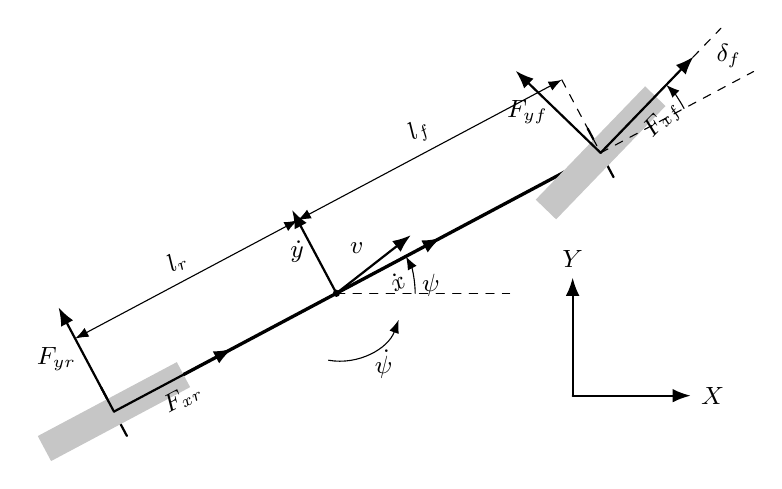
\begin{tikzpicture}[
    >=Latex,
    line cap=round,
    line join=round,
    font=\small
]

% -----------------------
% Parameters
% -----------------------
\def\psival{28}
\def\deltaval{18}
\def\lr{3.2}
\def\lf{3.8}

% -----------------------
% Coordinates
% -----------------------
\coordinate (R) at (0,0);
\coordinate (C) at ($(R)+({\psival}:\lr)$);
\coordinate (F) at ($(C)+({\psival}:\lf)$);

\coordinate (Fbody)  at ($(F)+({\psival}:1.6)$);
\coordinate (Fsteer) at ($(F)+({\psival+\deltaval}:1.6)$);

% -----------------------
% Body
% -----------------------
\draw[very thick] (R) -- (F);

% Axles
\draw[thick] ($(R)+({\psival+90}:0.35)$) -- ($(R)+({\psival-90}:0.35)$);
\draw[thick] ($(F)+({\psival+90}:0.35)$) -- ($(F)+({\psival-90}:0.35)$);

% -----------------------
% Wheels
% -----------------------
\begin{scope}[shift={(R)}, rotate=\psival]
    \fill[gray!45] (-1.0,-0.18) rectangle (1.0,0.18);
\end{scope}

\begin{scope}[shift={(F)}, rotate={\psival+\deltaval}]
    \fill[gray!45] (-1.0,-0.18) rectangle (1.0,0.18);
\end{scope}

% -----------------------
% Distances
% -----------------------
\draw[dashed] ($(R)+({\psival+90}:1.05)$) -- (R);
\draw[dashed] ($(C)+({\psival+90}:1.05)$) -- (C);
\draw[dashed] ($(F)+({\psival+90}:1.05)$) -- (F);

\draw[<->] ($(R)+({\psival+90}:1.05)$) -- node[above,sloped] {$l_r$} ($(C)+({\psival+90}:1.05)$);
\draw[<->] ($(C)+({\psival+90}:1.05)$) -- node[above,sloped] {$l_f$} ($(F)+({\psival+90}:1.05)$);

% -----------------------
% Center of gravity
% -----------------------
\fill (C) circle (1.3pt);

% -----------------------
% Velocities
% -----------------------
\draw[->,thick] (C) -- node[below,sloped] {$\dot{x}$} ($(C)+({\psival}:1.5)$);
\draw[->,thick] (C) -- node[left] {$\dot{y}$} ($(C)+({\psival+90}:1.2)$);

% v vector (correct direction)
\draw[->,thick] (C) -- node[above left] {$v$} ($(C)+({\psival+10}:1.2)$);

% -----------------------
% Reference axis
% -----------------------
\draw[dashed] (C) -- ++(2.2,0);

% -----------------------
% PSI angle (ONLY LABEL MOVED)
% -----------------------
\draw[->] ($(C)+(1.0,0)$)
arc[start angle=0,end angle=\psival,radius=1.0];

% ✅ LOWERED LABEL (only change)
\node at ($(C)+(1.2,0.10)$) {$\psi$};

% -----------------------
% Yaw rate
% -----------------------
\draw[->] ($(C)+(-0.1,-0.85)$)
arc[start angle=-100,end angle=-20,radius=0.8];

\node at ($(C)+(0.6,-0.9)$) {$\dot{\psi}$};

% -----------------------
% Rear forces
% -----------------------
\draw[->,thick] (R) -- node[below,sloped] {$F_{xr}$} ($(R)+({\psival}:1.7)$);
\draw[->,thick] (R) -- node[left] {$F_{yr}$} ($(R)+({\psival+90}:1.5)$);

% -----------------------
% Front forces
% -----------------------
\draw[->,thick] (F) -- node[below,sloped] {$F_{xf}$} ($(F)+({\psival+\deltaval}:1.7)$);
\draw[->,thick] (F) -- node[left] {$F_{yf}$} ($(F)+({\psival+\deltaval+90}:1.5)$);

% -----------------------
% Steering reference lines
% -----------------------
\draw[dashed] (F) -- ($(F)+({\psival}:2.2)$);
\draw[dashed] (F) -- ($(F)+({\psival+\deltaval}:2.2)$);

% -----------------------
% Delta angle
% -----------------------
\pic[
    draw,
    ->,
    "$\delta_f$",
    angle eccentricity=1.7,
    angle radius=12mm
] {angle = Fbody--F--Fsteer};

% -----------------------
% ✅ GLOBAL FRAME (VISIBLE FIX)
% -----------------------
\coordinate (G) at ($(C)+(3,-1.3)$);

\draw[->,thick] (G) -- ++(1.5,0) node[right] {$X$};
\draw[->,thick] (G) -- ++(0,1.5) node[above] {$Y$};

\end{tikzpicture}
\caption{Bicycle model representation for a mining dump truck.}
\label{fig:bicycle_model_dump_truck}
\end{figure}

\begin{equation}
\ddot{y}
=
\left(
\frac{C_r l_r - C_f l_f}{m \dot{x}}
-
\dot{x}
\right)\dot{\psi}
-
\left(
\frac{C_f + C_r}{m \dot{x}}
\right)\dot{y}
+
\frac{C_f}{m}\,\delta_f
\end{equation}

\begin{equation}
\ddot{\psi}
=
-
\left(
\frac{C_f l_f^2 + C_r l_r^2}{I_z \dot{x}}
\right)\dot{\psi}
+
\left(
\frac{C_r l_r - C_f l_f}{I_z \dot{x}}
\right)\dot{y}
+
\frac{C_f l_f}{I_z}\,\delta_f
\end{equation}

\begin{equation}
\dot{Y}
=
\dot{x} \sin\psi + \dot{y}\cos\psi
\approx
\dot{x}\psi + \dot{y}
\end{equation}

The lateral tire forces are modeled using a linear tire model, where the lateral force is proportional to the slip angle:
\begin{equation}
F_{yf} = C_f \alpha_f, \qquad F_{yr} = C_r \alpha_r
\end{equation}

Under the small-angle assumption, the slip angles can be approximated as:
\begin{equation}
\alpha_f \approx \delta_f - \frac{\dot{y} + l_f \dot{\psi}}{\dot{x}},
\qquad
\alpha_r \approx -\,\frac{\dot{y} - l_r \dot{\psi}}{\dot{x}}
\end{equation}

The lateral dynamic model is described by a set of states associated with the planar motion of the vehicle. In particular, the system states are the lateral velocity $\dot{y}$, the yaw rate $\dot{\psi}$, the yaw angle $\psi$, and the global lateral displacement $Y$. The longitudinal velocity $\dot{x}$ is treated as a measurable scheduling variable and is assumed to remain constant or slowly varying over the prediction horizon. The steering angle at the front axle, $\delta_f$, is considered the control input. The physical parameters of the model are given by the vehicle mass $m$, the yaw moment of inertia $I_z$, the distances $l_f$ and $l_r$ from the center of gravity to the front and rear axles, and the tire cornering stiffness coefficients $C_f$ and $C_r$. The lateral tire forces at the front and rear axles are denoted by $F_{yf}$ and $F_{yr}$, respectively, while $F_{xf}$ and $F_{xr}$ represent the longitudinal tire forces. The tire slip angles, $\alpha_f$ and $\alpha_r$, are introduced to model the lateral tire behavior through a linear tire approximation valid under small slip-angle conditions.

\begin{table}[htbp]
\centering
\caption{Definition of variables and parameters used in the lateral dynamic model.}
\label{tab:model_variables}
\begin{tabular}{ll}
\hline
Symbol & Definition \\
\hline
$\dot{x}$      & Longitudinal velocity of the vehicle \\
$\dot{y}$      & Lateral velocity at the center of gravity (CG) \\
$\ddot{y}$     & Lateral acceleration \\
$\psi$         & Yaw angle (vehicle heading angle) \\
$\dot{\psi}$   & Yaw rate \\
$\ddot{\psi}$  & Yaw acceleration \\
$Y$            & Global lateral position \\
$\dot{Y}$      & Global lateral velocity \\
$\delta_f$     & Front steering angle (control input) \\
$m$            & Total vehicle mass \\
$I_z$          & Yaw moment of inertia about the vertical axis \\
$l_f$          & Distance from the CG to the front axle \\
$l_r$          & Distance from the CG to the rear axle \\
$C_f$          & Front tire cornering stiffness \\
$C_r$          & Rear tire cornering stiffness \\
$F_{yf}$       & Front lateral tire force \\
$F_{yr}$       & Rear lateral tire force \\
$F_{xf}$       & Front longitudinal tire force \\
$F_{xr}$       & Rear longitudinal tire force \\
$\alpha_f$     & Front tire slip angle \\
$\alpha_r$     & Rear tire slip angle \\
$v$            & Resultant vehicle speed at the CG \\
\hline
\end{tabular}
\end{table}

% \subsection{Flat Output Definition}

% A nonlinear system is said to be differentially flat if there exists an output vector $z$ such that all states and inputs can be expressed in terms of $z$ and a finite number of its derivatives.

% For the planar bicycle model, we select the flat output as
% \begin{equation}
% z =
% \begin{bmatrix}
% X \\
% Y
% \end{bmatrix}.
% \end{equation}

% \subsection{State and Input Parametrization}

% We demonstrate that all system states and inputs can be expressed as functions of the flat output and its derivatives.

% \paragraph{Heading angle}
% From the kinematic equations,
% \begin{equation}
% \tan\psi = \frac{\dot{Y}}{\dot{X}},
% \end{equation}
% thus,
% \begin{equation}
% \psi = \text{atan2}(\dot{Y}, \dot{X}).
% \end{equation}

% \paragraph{Longitudinal velocity}
% \begin{equation}
% v = \sqrt{\dot{X}^2 + \dot{Y}^2}.
% \end{equation}

% \paragraph{Curvature}
% Differentiating $\psi$, the yaw rate is given by
% \begin{equation}
% \dot{\psi} =
% \frac{\dot{X}\ddot{Y} - \dot{Y}\ddot{X}}
% {\dot{X}^2 + \dot{Y}^2}.
% \end{equation}

% The curvature is then
% \begin{equation}
% \kappa =
% \frac{\dot{\psi}}{v}
% =
% \frac{\dot{X}\ddot{Y} - \dot{Y}\ddot{X}}
% {(\dot{X}^2 + \dot{Y}^2)^{3/2}}.
% \end{equation}

% \paragraph{Steering angle}
% Using the bicycle model relationship,
% \begin{equation}
% \kappa = \frac{\tan\delta_f}{L},
% \end{equation}
% the steering input is obtained as
% \begin{equation}
% \delta_f = \arctan(L \kappa).
% \end{equation}

% Therefore, all states $(X,Y,\psi,v)$ and inputs $(\delta_f)$ can be parametrized by the flat output $z = [X, Y]^T$ and its derivatives. This proves that the system is differentially flat.

% \subsection{Trajectory Generation}

% Given a desired path $(X_d(t), Y_d(t))$, the corresponding reference signals are computed as
% \begin{align}
% \psi_d &= \text{atan2}(\dot{Y}_d, \dot{X}_d), \\
% v_d &= \sqrt{\dot{X}_d^2 + \dot{Y}_d^2}, \\
% \kappa_d &=
% \frac{\dot{X}_d \ddot{Y}_d - \dot{Y}_d \ddot{X}_d}
% {(\dot{X}_d^2 + \dot{Y}_d^2)^{3/2}}, \\
% \delta_{ff} &= \arctan(L \kappa_d).
% \end{align}

% Thus, the flatness property allows direct computation of feedforward control inputs from the desired trajectory.

% \subsection{Dynamic Tracking Control Design}

% To account for vehicle dynamics, the yaw dynamics of the mining truck are considered in the form
% \begin{equation}
% \ddot{\psi} = A \dot{\psi} + B \dot{y} + C \delta_f,
% \end{equation}
% where $A$, $B$, and $C$ are defined as
% \begin{align}
% A &= -\frac{C_f l_f^2 + C_r l_r^2}{I_z v_x}, \\
% B &= \frac{C_r l_r - C_f l_f}{I_z v_x}, \\
% C &= \frac{C_f l_f}{I_z}.
% \end{align}

% Using the kinematic approximation
% \begin{equation}
% \dot{y} \approx \dot{Y} - v_x \psi,
% \end{equation}
% the control law is obtained via feedback linearization.

% \subsection{Feedback Linearization Controller}

% Define the tracking error
% \begin{equation}
% e_\psi = \psi - \psi_d, \qquad
% e_{\dot{\psi}} = \dot{\psi} - \dot{\psi}_d.
% \end{equation}

% Enforcing second-order error dynamics
% \begin{equation}
% \ddot{e}_\psi + k_1 \dot{e}_\psi + k_0 e_\psi = 0,
% \end{equation}
% leads to the desired yaw acceleration
% \begin{equation}
% \nu_\psi =
% \ddot{\psi}_d
% - k_1 (\dot{\psi} - \dot{\psi}_d)
% - k_0 (\psi - \psi_d).
% \end{equation}

% Solving for the steering input yields
% \begin{equation}
% \delta_f =
% \frac{1}{C}
% \left[
% \nu_\psi
% - A \dot{\psi}
% - B (\dot{Y} - v_x \psi)
% \right].
% \end{equation}

% \subsection{Lateral Error Compensation}

% To improve path tracking, the lateral error is defined as
% \begin{equation}
% e_y = -\sin\psi_d (X - X_d) + \cos\psi_d (Y - Y_d).
% \end{equation}

% The control law is augmented as
% \begin{equation}
% \delta_f =
% \frac{1}{C}
% \left[
% \ddot{\psi}_d
% - k_1 e_{\dot{\psi}}
% - k_0 e_\psi
% - k_y e_y
% - A \dot{\psi}
% - B (\dot{Y} - v_x \psi)
% \right].
% \end{equation}

% This control law combines feedforward trajectory generation from differential flatness with feedback stabilization based on the dynamic bicycle model.


\subsection{Differential Flatness-Based Reference Generation}

The planar motion of the vehicle can be described using a kinematic bicycle model, which is known to be differentially flat. A nonlinear system is said to be differentially flat if there exists an output vector $z$ such that all system states and inputs can be expressed as functions of $z$ and a finite number of its derivatives.

For the planar vehicle model, the flat output is selected as
\begin{equation}
z =
\begin{bmatrix}
X \\
Y
\end{bmatrix}.
\end{equation}

All relevant states and inputs can be reconstructed from the flat output as follows:

\paragraph{Heading angle}
\begin{equation}
\psi = \text{atan2}(\dot{Y}, \dot{X})
\end{equation}

\paragraph{Longitudinal velocity}
\begin{equation}
v = \sqrt{\dot{X}^2 + \dot{Y}^2}
\end{equation}

\paragraph{Path curvature}
\begin{equation}
\kappa =
\frac{\dot{X}\ddot{Y} - \dot{Y}\ddot{X}}
{(\dot{X}^2 + \dot{Y}^2)^{3/2}}
\end{equation}

\paragraph{Steering angle}
\begin{equation}
\delta_{ff} = \arctan(L \kappa)
\end{equation}

This formulation enables direct generation of dynamically feasible trajectories and the corresponding feedforward steering input from a desired path.

\subsection{Reference Trajectory Generation: Lane Change}

To evaluate the proposed controller, a smooth lane-change maneuver is selected as the reference trajectory. The longitudinal motion is defined as
\begin{equation}
X_d(t) = v_x t
\end{equation}

The lateral displacement is defined using a normalized cubic polynomial that ensures smooth transitions:
\begin{equation}
Y_d(t) = y_f \left(3\tau^2 - 2\tau^3\right), \quad \tau = \frac{t}{T}
\end{equation}

where $y_f$ is the desired lateral displacement and $T$ is the maneuver duration.

The first and second derivatives are given by:
\begin{align}
\dot{Y}_d(t) &= y_f \left(\frac{6\tau}{T} - \frac{6\tau^2}{T}\right) \\
\ddot{Y}_d(t) &= y_f \left(\frac{6}{T^2} - \frac{12\tau}{T^2}\right)
\end{align}

The desired heading, yaw rate, and yaw acceleration are computed directly from the flat outputs:
\begin{align}
\psi_d &= \text{atan2}(\dot{Y}_d, \dot{X}_d) \\
\dot{\psi}_d &= \frac{\dot{X}_d \ddot{Y}_d - \dot{Y}_d \ddot{X}_d}{\dot{X}_d^2 + \dot{Y}_d^2}
\end{align}

The corresponding feedforward steering command is obtained as:
\begin{equation}
\delta_{ff} = \arctan(L \kappa_d)
\end{equation}


\subsection{Flatness-Based Tracking Control with Integral Action}

To account for model uncertainties and achieve accurate trajectory tracking, a feedback linearization controller augmented with lateral error integral action is proposed.

The yaw dynamics can be expressed as:
\begin{equation}
\ddot{\psi} = A \dot{\psi} + B \dot{y} + C \delta_f
\end{equation}

Using the kinematic approximation:
\begin{equation}
\dot{y} \approx \dot{Y} - v_x \psi
\end{equation}

the system is reformulated explicitly in terms of measurable states.

\paragraph{Error definitions}

\begin{align}
e_\psi &= \psi - \psi_d \\
e_{\dot{\psi}} &= \dot{\psi} - \dot{\psi}_d \\
e_y &= -\sin(\psi_d)(X - X_d) + \cos(\psi_d)(Y - Y_d)
\end{align}

To compensate for steady-state errors caused by model mismatch, an integral term is introduced:
\begin{equation}
e_y^{int} = \int e_y(t) \, dt
\end{equation}

\paragraph{Control law}

The final steering input is defined as:
\begin{equation}
\boxed{
\begin{aligned}
\delta_f =\;& \delta_{ff} + \frac{1}{C} \Big[ \ddot{\psi}_d 
- k_1 e_{\dot{\psi}} - k_0 e_\psi - k_y e_y \\
&- k_i e_y^{int}
- A \dot{\psi}
- B (\dot{Y} - v_x \psi)
\Big]
\end{aligned}
}
\end{equation}

\paragraph{Control interpretation}

The proposed controller combines three key components:

\begin{itemize}
\item Feedforward term $\delta_{ff}$ derived from differential flatness, capturing path curvature.
\item Feedback linearization terms that cancel vehicle dynamics and enforce desired error dynamics.
\item Integral action on lateral error to eliminate steady-state offsets due to modeling inaccuracies.
\end{itemize}

This structure enables accurate trajectory tracking with reduced computational complexity compared to optimization-based controllers such as MPC.


\subsection{Active Disturbance Rejection Control}
\label{sec:adrc}

Mining vehicles operate under highly variable conditions: load changes, uneven terrain, and uncertainty in tire-soil friction. ADRC addresses this by treating all unknown dynamics as a \emph{total disturbance}, estimated and canceled in real time via an Extended State Observer (ESO), without requiring an accurate system model.

\subsubsection{Extended State Observer} 

The ESO estimates the global lateral position, its derivative, and the total disturbance:
%
\begin{equation}
z_1 = \hat{Y},\quad z_2 = \dot{\hat{Y}},\quad z_3 = \hat{f}
\label{eq:eso_states}
\end{equation}

The discrete-time observer equations are:
%
\begin{equation}
    e = Y_m - z_1 
\end{equation}

\begin{equation}
    \begin{aligned}
        \dot{z}_1 &= z_2 + \beta_1 e \\
        \dot{z}_2 &= z_3 + \beta_2 e + b_0\delta_f\\
        \dot{z}_3 &= \beta_3 e 
    \end{aligned}
\end{equation}


%
where each state is integrated with sampling period $T_s$:
%
\begin{equation}
z_i(t + T_s) = z_i(t) + T_s\,\dot{z}_i
\label{eq:eso_integration}
\end{equation}

The observer gains are obtained via bandwidth parameterization:
%
\begin{equation}
\beta_1 = 3\omega_o,\quad \beta_2 = 3\omega_o^2,\quad \beta_3 = \omega_o^3
\label{eq:eso_gains}
\end{equation}

\subsection{Control Law}

The control signal is computed as:
%
\begin{equation}
u_0 = k_p(Y_d - z_1) + k_d(0 - z_2)
\label{eq:adrc_u0}
\end{equation}
%
\begin{equation}
    \boxed{
\delta_f = \frac{u_0 - z_3}{b_0}
    }
\label{eq:adrc_control}
\end{equation}
%
with $b_0 = C_f/m$, $k_p = \omega_c^2$, $k_d = 2\omega_c$, and $\omega_c \leq \omega_o/2$.
%%%%%%%%%%%%%%%%%%%%%%%%%%%%%%%%%%%%%%%%%%%%%%%%%%%%%%%%%%%%%%%%%%%%%%%%
\subsection{Sliding Mode Control with Quasi-Continuous Approximation}

The lateral dynamics of the vehicle can be expressed in the input--output form as

\begin{equation}
\ddot{y}=f(x)+g(x)\delta_f
\end{equation}

where $f(x)$ and $g(x)$ represent nonlinear functions of the system states, and $\delta_f$ denotes the steering input. The control objective is to ensure convergence of the lateral position $y$ to the desired trajectory $y_d$.

\subsubsection{Error Definition}

The lateral tracking error is defined as

\begin{equation}
e_y = y-y_d
\end{equation}

and the sliding surface is selected as

\begin{equation}
\sigma = \dot{e}_y + \lambda e_y
\end{equation}

where $\lambda>0$ is a design parameter that determines the convergence rate of the tracking error.

\subsubsection{Control Law}

To reduce chattering while preserving the robustness properties of sliding mode control, a quasi-continuous approximation based on the hyperbolic tangent function is employed. The resulting steering control law is given by

\begin{equation}
\boxed{
\begin{aligned}
\delta_f=\frac{m}{C_f}\Bigg(&-\ddot{x}\psi-\frac{C_r l_r-C_f l_f}{m\dot{x}}\dot{\psi}+\frac{C_f+C_r}{m\dot{x}}\dot{y}\\
&+\ddot{y}_d-\lambda_2\dot{e}-k_1\tanh\left(\frac{\sigma}{\nu}\right)\Bigg)
\end{aligned}
}
\end{equation}

where $k>0$ is the switching gain and $\nu>0$ defines the thickness of the boundary layer around the sliding surface.
%%%%%%%%%%%%%%%%%%%%%%%%%%%%%%%%%%%%%%%%%%%%%%%%%%%%%%%%%%%%%%%%%%%%%%%%%%%%%%%%%
\section{Simulation Results}

The performance of the proposed flatness-based controller is evaluated using a lane-change maneuver with a target lateral displacement of $y_f = 3.5$ m.

\subsection{Tracking Performance}

Fig.~\ref{fig:lane_change_tracking} shows the lateral displacement tracking results. The controller achieves accurate trajectory tracking with zero steady-state error, demonstrating successful convergence to the desired path. The transient response is smooth and stable, with no oscillatory behavior.

An initial rapid increase in lateral displacement is observed, driven by the feedforward component obtained from trajectory curvature. This is followed by a slower convergence phase associated with the feedback and integral actions, which compensate for model mismatch and dynamic uncertainties.

\subsection{Role of Control Components}

The results highlight the contribution of each element of the proposed control structure:

\begin{itemize}
\item The feedforward term derived from differential flatness provides the baseline steering action required to follow the path geometry.
\item Feedback linearization compensates for nonlinear vehicle dynamics and ensures stable transient behavior.
\item Integral action eliminates steady-state lateral error caused by modeling inaccuracies and approximations.
\end{itemize}

Without integral action, the controller exhibits a persistent steady-state tracking error despite achieving correct heading alignment. The inclusion of the integral term enables complete error rejection.

\subsection{Discussion}

The simulation results demonstrate that the proposed flatness-based controller can achieve high-quality trajectory tracking for heavy-duty vehicles. The controller maintains stability and smoothness while accurately following the desired path.

These results indicate that flatness-based control, combined with feedback linearization and integral correction, provides an effective and computationally efficient alternative to optimization-based approaches for structured, low-speed mining scenarios.

\begin{figure}[htbp]
\centering
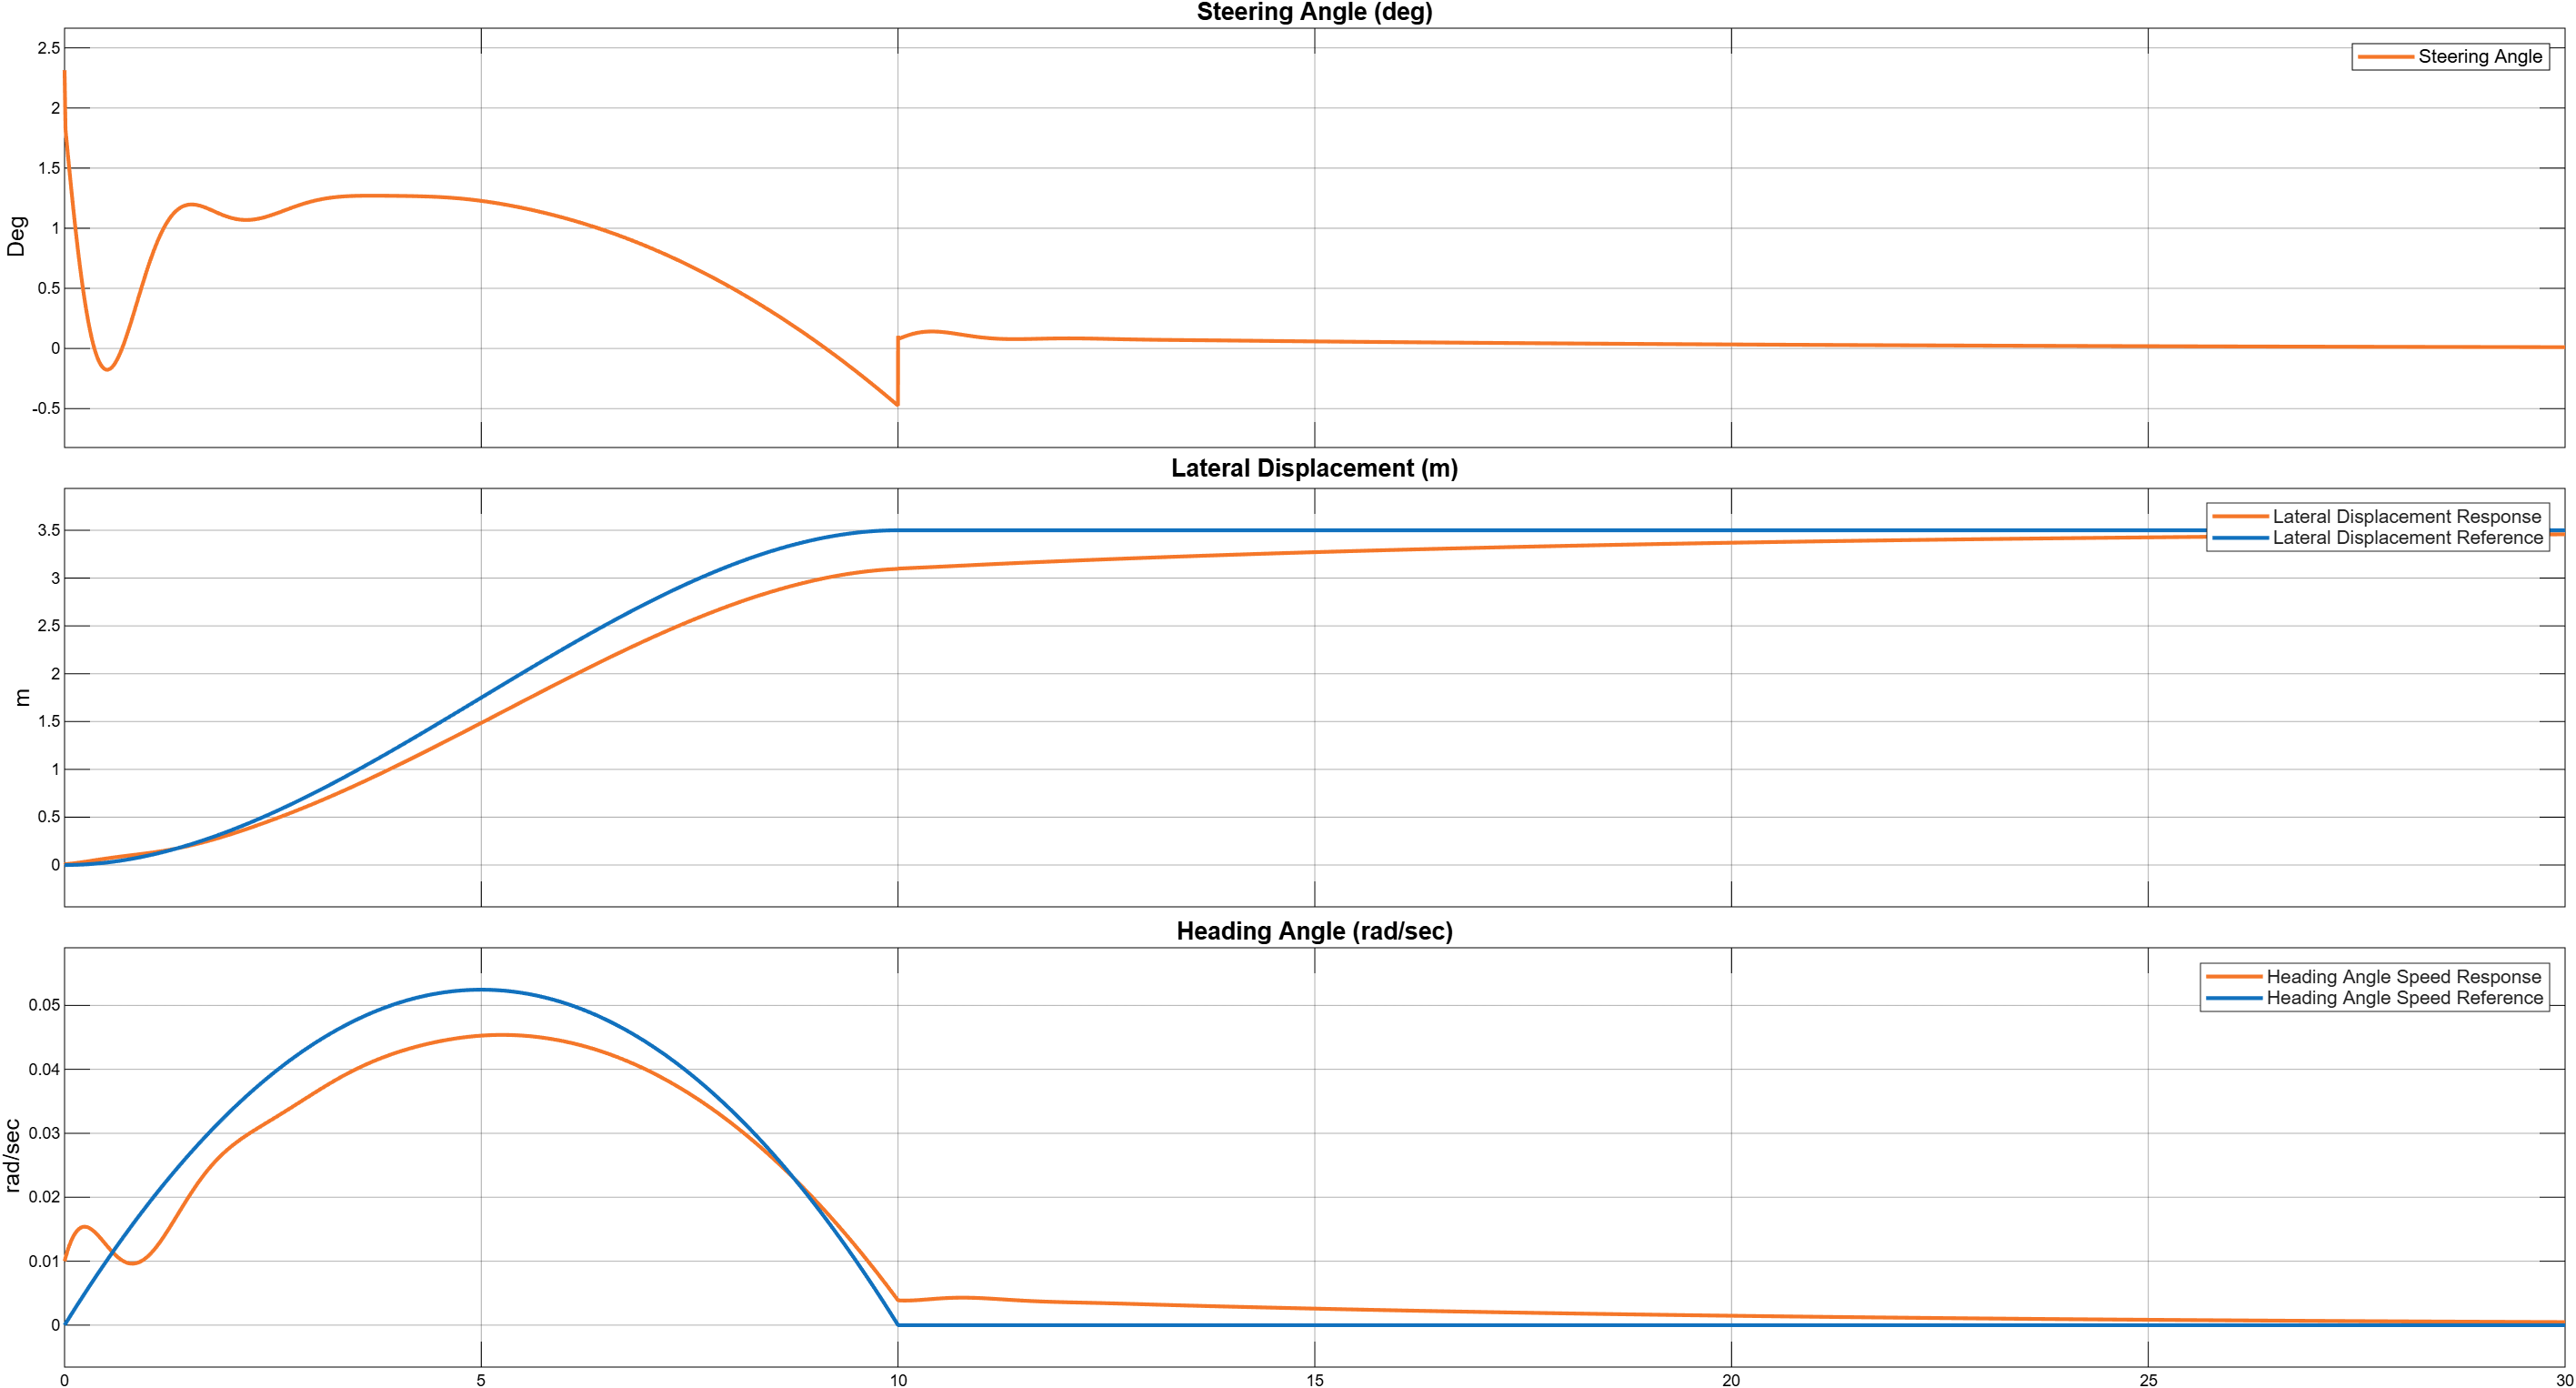
\includegraphics[width=1\linewidth]{lane_change_tracking.png}
\caption{Lateral displacement tracking performance for the lane-change maneuver. The proposed controller achieves accurate tracking with zero steady-state error.}
\label{fig:lane_change_tracking}
\end{figure}

The simulation results show that the ADRC controller achieves accurate trajectory tracking without requiring an exact dynamic model. The Extended State Observer estimates and compensates for the total disturbance, which encompasses model uncertainties, terrain irregularities, and payload variations. A slight response delay is observed due to the observer convergence time, an inherent characteristic of the ESO that can be mitigated by increasing the observer bandwidth $\omega_o$ at the expense of higher noise sensitivity. Despite this limitation, the controller maintains stability and achieves zero steady-state error, offering a robust and computationally lightweight alternative to optimization-based methods.

\begin{figure}[htbp]
\centering
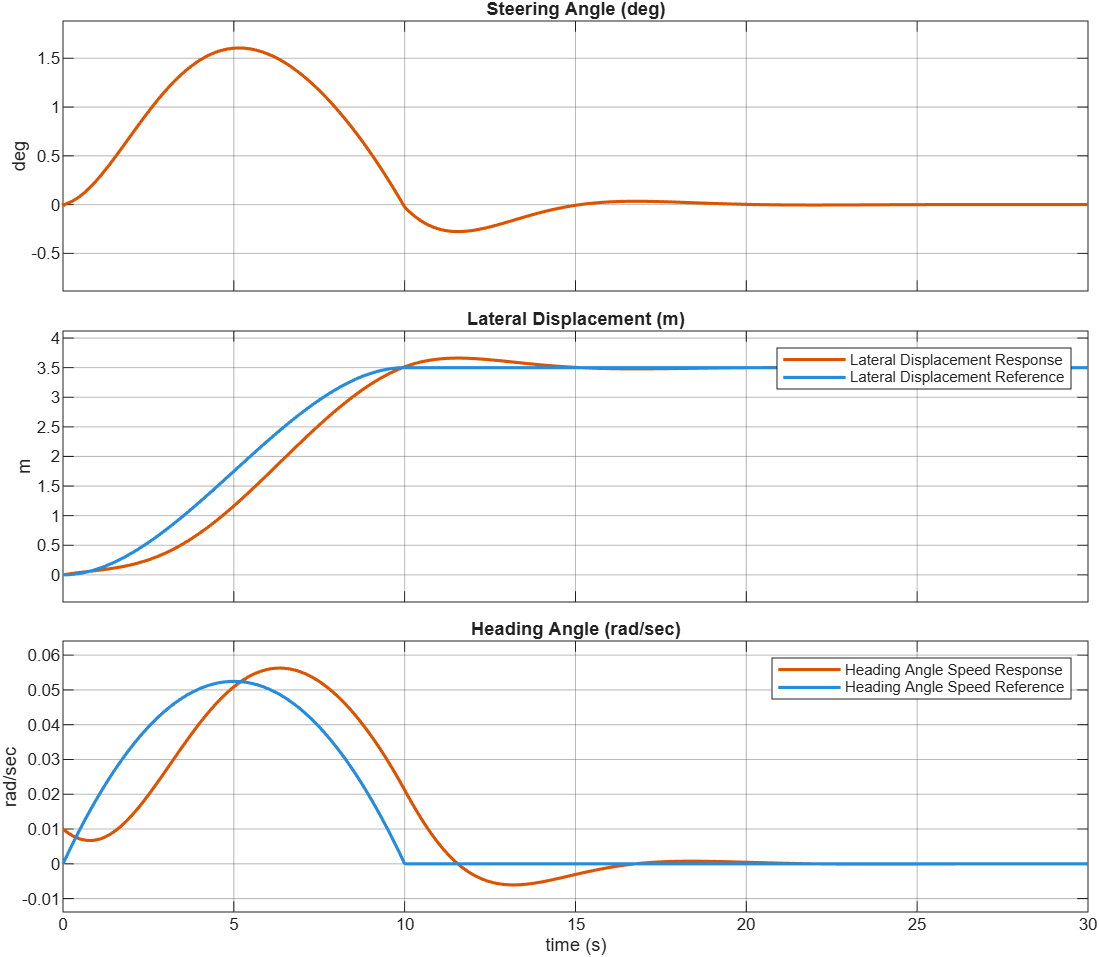
\includegraphics[width=1\linewidth]{ADRC.png}
\caption{Lateral displacement tracking performance for the lane-change maneuver using the ADRC-based controller. The ADRC achieves accurate tracking with zero steady-state error despite model uncertainties and external disturbances.}
\label{fig:ADRC}
\end{figure}

\begin{thebibliography}{xx}

\bibitem[Lee et~al.(2008)]{refFullVehicleModel}
J.~Lee, J.~Lee, and S.-J. Heo.
\newblock ``Full vehicle dynamic modeling for chassis control.''
\newblock In \emph{FISITA World Automotive Congress}, 2008.

\bibitem[Kebbati et~al.(2023)]{refVehicleControlReview}
Y.~Kebbati, N.~Ait-Oufroukh, D.~Ichalal, and V.~Vigneron.
\newblock ``Lateral control for autonomous wheeled vehicles: a technical review.''
\newblock \emph{Asian Journal of Control}, vol.~25, no.~4, pp.~2539--2563, 2023.

\bibitem[Berglund et~al.(2010)]{refBSpline}
T.~Berglund, A.~Brodnik, H.~Jonsson, M.~Staffanson, and I.~S\"oderkvist.
\newblock ``Planning smooth and obstacle-avoiding B-spline paths for autonomous mining vehicles.''
\newblock \emph{IEEE Transactions on Automation Science and Engineering}, vol.~7, no.~1, pp.~167--172, 2010.

\bibitem[Li and Zhan(2018)]{refIntelligentMining}
J.~Li and K.~Zhan.
\newblock ``Intelligent mining technology for an underground metal mine based on unmanned equipment.''
\newblock \emph{Engineering}, vol.~4, pp.~381--391, 2018.

\bibitem[Chen et~al.(2023)]{refChen2023}
L.~Chen, Z.~Qin, M.~Hu, H.~Gao, et al.
\newblock ``Trajectory tracking control of autonomous heavy-duty mining dump trucks with uncertain dynamic characteristics.''
\newblock \emph{Science China Information Sciences}, vol.~66, 2023.

\bibitem[Lalezar et~al.(2024)]{refIFACDumpTruck}
M.~Lalezar, I.~Izadi, S.~H. Hoseinie, and H.~Mohamadrezaie.
\newblock ``A model predictive control algorithm for autonomous mining dump trucks.''
\newblock \emph{IFAC PapersOnLine}, vol.~58, no.~22, pp.~60--65, 2024.

\bibitem[GlobalData(2026)]{ref1}
GlobalData.
\newblock \emph{Latin America Mining Review 2026}.
\newblock GlobalData, Apr. 2026.
\newblock [Online]. Available: \url{https://www.globaldata.com/store/report/latin-america-mining-analysis/}

\bibitem[International Trade Administration(2025)]{ref2}
International Trade Administration.
\newblock \emph{Chile -- Mining}.
\newblock U.S. Department of Commerce, Nov. 24, 2025.
\newblock [Online]. Available: \url{https://www.trade.gov/country-commercial-guides/chile-mining}

\bibitem[Hernandez and Perez(2024)]{ref3}
C.~Hernandez and A.~Perez.
\newblock \emph{The State of Mining in Latin America}.
\newblock FCAP Advisors, Jun. 11, 2024.
\newblock [Online]. Available: \url{https://www.fcapadvisors.com/post/the-state-of-mining-in-latin-america}

\bibitem[Statista(2025)]{ref4}
Statista.
\newblock \emph{Mining in Chile -- Statistics \& Facts}.
\newblock Dec. 17, 2025.
\newblock [Online]. Available: \url{https://www.statista.com/topics/6550/mining-in-chile/}

\bibitem[Bujakiewicz(2025)]{ref5}
B.~Bujakiewicz.
\newblock ``El 31\% de las empresas mineras de Latinoam\'erica apuesta a la IA para optimizar operaciones.''
\newblock \emph{Infobae}, Sep. 25, 2025.
\newblock [Online]. Available: \url{https://www.infobae.com/america/ciencia-america/2025/09/25/el-31-de-las-empresas-mineras-de-latinoamerica-apuesta-a-la-ia-para-optimizar-operaciones/}

\bibitem[Digital Market Latin America(2024)]{ref6}
Digital Market Latin America.
\newblock ``La miner\'ia inteligente impulsa la transformaci\'on tecnol\'ogica en Am\'erica Latina.''
\newblock Sep. 4, 2024.
\newblock [Online]. Available: \url{https://digitalmarketla.com/web/2024/09/04/la-mineria-inteligente-impulsa-la-transformacion-tecnologica-en-america-latina/}

\end{thebibliography}

%\appendix
%\section{A summary of Latin grammar}
%\section{Some Latin vocabulary}

\appendix
\section{CAT 797 Specification}

Using the standard bicycle model approximations, the distances from the center of gravity to the front and rear axles, as well as the yaw moment of inertia, are obtained as:

\begin{equation}
l_f = L \left( 1 - \frac{m_f}{m} \right), \quad
l_r = L \left( 1 - \frac{m_r}{m} \right), \quad
I_z = l_f \, l_r \, m
\end{equation}

For the Caterpillar 797F dump truck, the following parameters are used:

\begin{align}
L &= 7.195 \ \text{m} \\
\frac{m_f}{m} &= 0.333, \quad \frac{m_r}{m} = 0.667 \\
m &= 623{,}690 \ \text{kg}
\end{align}

Substituting into the equations:
s
\begin{align}
l_f &= 7.195 \times (1 - 0.333) = 4.80 \ \text{m} \\
l_r &= 7.195 \times (1 - 0.667) = 2.40 \ \text{m} \\
I_z &= 4.80 \times 2.40 \times 623{,}690 \approx 7.19 \times 10^{6} \ \text{kg} \cdot \text{m}^2
\end{align}

\subsection{Cornering Stiffness Parameters}

Unlike geometric parameters, the cornering stiffness coefficients cannot be directly derived from manufacturer data. Therefore, they are estimated using a data-driven least squares method. Additionally, simulation-based estimates obtained from the CARLA environment are used to capture terrain-dependent variations, providing a more realistic representation of tire-road interaction in mining environments.

\end{document}